%! TeX root: ../thesis_a4.tex

\chapter{Music and scientific background}
\label{ch02_sb}

Computational musicology is a pivotal discipline for analyzing and understanding musical traditions, leveraging algorithms to uncover musical structures and patterns. While \acrfull{DL} has established as the leading technology for many problems in the fields of \acrfull{MIR} and \acrfull{ASP}, the practical application of \acrshort{DL} in computational musicology pipelines remains limited; \acrshort{DL} systems often offer limited interpretability and control, and there is a scarcity of methodologies explicitly tailored to the musical structures and performance practices of under-studied repertoires.
%
%it is not clear how to integrate these techniques into musicological studies due to the limited interpretability and control, but most importantly, because of the scarcity of methodologies tailored to the musical structures and practices of diverse repertoires. 
%Nonetheless, an important body of research efforts have been carried out toward developing computational methodologies for the analysis and understanding of particular musical repertoires.
Additionally, many music traditions suffer from a lack of large, high-quality, annotated datasets. Nevertheless, a growing body of work is emerging to bridge this gap, aiming at developing computational tools to study the unique characteristics of specific musical repertoires.
%
This chapter introduces the reader to the scientific background with a critical view, aiming to present the literature where this dissertation is grounded and the current challenge, and it is partly based on the discussions in this publication:

\begin{mybox}{FRSM 2022}
    Genís Plaja-Roglans, Thomas Nuttall, Xavier Serra \& Marius Miron (2022).
    \emph{Continuing CompMusic: new approaches in the computational analysis of Carnatic music}.
    In: Proc. of 27th Int. Symposium on Frontiers of Research in Speech and Music (FRSM), Online.  %, Advances in Intelligent Systems and Computing.
 \end{mybox}


First, Section~\ref{ch02_sb:sec:carnatic} provides a basic introduction to Carnatic music, the art music style that we utilize as case study in this thesis, covering the fundamental concepts of the repertoire. Because the focus of this dissertation is placed on the melodic analysis of Carnatic music, we emphasize the melodic concepts, performance format, and instrumentation.
%
Subsequently, Section~\ref{ch02_sb:sec:computational-carnatic} reviews the literature on computational analysis of the Carnatic and Hindustani repertoires,\footnote{Note that, alongside Hindustani music, Carnatic music constitutes one of the two main musical traditions of \acrfull{IAM}. Whilst these two art music traditions from India have been evolving separately for hundreds of years, they share core concepts and practices, and therefore are often studied jointly. For that reason, the prior work on the computational analysis of this music style cannot be understood without considering research efforts for Hindustani Music as well.} emphasizing melodic analysis tasks. Subsequently, we introduce the tasks of \acrfull{VME}–-in Section~\ref{ch02_sb:sec:pitch-extraction}–-and \acrfull{MSS} and \acrfull{SVE}–-in Section~\ref{ch02_sb:sec:music-source-separation}. For each task, we provide an overview of existing methods and current trends, present the standard evaluation metrics, and discuss the limitations of these tasks in the context of the computational analysis of Carnatic music.


%Section~\ref{ch02_sb:sec:pitch-extraction} reviews the literature on \acrfull{VME} and Section~\ref{ch02_sb:sec:music-source-separation} presents existing systems and current challenges for \acrfull{MSS} and \acrfull{SVE}. In these sections, the evaluation metrics are presented and discussed, and 
%These sections also include an overview of the current limitations of these tasks in the context of the computational analysis of Carnatic Music is given.
%



\section{Carnatic Music}\label{ch02_sb:sec:carnatic}
Carnatic music (in sanskrit: Kar\d{n}\={a}\d{t}aka Sa\.{n}g\={\i}ta) is a prominent art music style that originated in the royal courts and temples of South India and is still performed today in concert halls and temple festivals. With its fan base encompassing millions of listeners and practitioners around the globe~\citep{gulati-mining}, the interest in computational approaches for analyzing and understanding Carnatic music has grown in recent years~\citep{tzanetakis-ethnomusicology}. This section is aimed at providing the reader with a basic introduction to Carnatic music, focusing on the most relevant concepts and practices for this dissertation. 
%
The scope is set on instrumentation, performance, and especially melodic aspects, which are particularly interesting aspects for our work.
%
The text in this section is based on Dr. Lara Pearson's and Dr. Brindha Manickavasakan's introduction in the Tutorial on Computational Analysis of Carnatic and Hindustani Music presented at ISMIR 2022 in Bengaluru, India, which the candidate of this thesis co-authored.\footnote{To re-use text portions of Section~\ref{ch02_sb:sec:carnatic} please acknowledge Dr. Pearson and Dr. Manickavasakan's text in the tutorial: \url{https://mtg.github.io/IAM-tutorial-ismir22}}
%
For an extensive introduction to Carnatic Music please refer to~\citep{carnatic-book}.


\subsection{Musical format and instrumentation}
In contemporary Carnatic music performances, the predominant format features a lead vocalist, either solo or in a vocal ensemble (three singers in the center front for the example in Figure~\ref{fig:ch02:carnatic-performance}). The vocalist is typically accompanied by a violinist (found in the left in Figure~\ref{fig:ch02:carnatic-performance}), who mirrors the vocal line either in unison or at the octave, resulting in a predominantly monophonic melodic texture. However, during improvisational segments
%—collectively known as manodharma saṅgīta—
the violinist often engages in responsive interplay, echoing and elaborating upon the phrases sung by the vocalist. This dynamic interaction introduces a heterophonic texture, enriching the musical tapestry with nuanced and expressive variations.


%mṛdaṅgam, %ghaṭam, %kañjīra, %tambūrā
The percussion section is normally led by a double-ended drum known as mridangam (in sanskrit \textit{m\d{r}da\.{n}gam}, found in the right in Figure~\ref{fig:ch02:carnatic-performance}), and it may include other percussion instruments such as the ghatam (clay pot, in sanskrit \textit{gha\d{t}am}), kanjira (small frame drum, in sanskrit \textit{kañjīra}), and morsing (mouth harp). Finally, an important feature is the tanpura drone played throughout. This can be performed using either the physical instrument, the tanpura (\textit{tamb\={u}r\={a}}), or an electronic imitation of the instrument, known as the shruti box. In the performance depicted in Figure~\ref{fig:ch02:carnatic-performance}, the drone is provided by the tanpura, which can be seen in the center behind the three vocalists.
%
%\textbf{Make footnote!} Implications for MIR: Notwithstanding the dominant monophonic melodic line, the overall instrumental texture is heterophonic, which is a challenge for predominant pitch extraction.


\begin{figure}[t]
    \centerline{
    \includegraphics[width=\columnwidth]{ch02_sb/figures/vocal_carnatic.jpg}}
    \caption{\textbf{A Carnatic music performance.} Led by the vocalists R.K. Shriramkumar, Amritha Murali, Ramakrishnan Murthy, accompanied by Madan Mohan on violin, Arunprakash Krishnan on mridangam and Nanditha Kannan on the tanpura. Photo by Rajappane Raju.}
    \label{fig:ch02:carnatic-performance}
\end{figure}



In Carnatic music, performance formats range from predominantly composed to highly improvisational. The former, known as \textit{kalpita sa\.{n}g\={\i}ta}, encompasses structured compositions, while the latter, termed \textit{manodharma sa\.{n}g\={\i}ta}, involves spontaneous creativity. However, the distinction is not absolute. Compositions often incorporate extemporaneous variations, and improvisational segments frequently draw upon established melodic phrases~\citep{ramanathan-sargam}. Moreover, compositions themselves originate from a composer's creative process, blending both composed and improvisational elements before becoming part of the fixed repertoire~\citep{nooshin-improvisation,pearson-improvisation}. Thus, both formats intertwine improvisation and composition, differing primarily in emphasis and execution.



\subsection{Melodic concepts.}
%\subsubsection{Rāga and rāga bhāva}
\paragraph*{R\={a}ga}
The melodic frameworks on which Carnatic music is based are known as r\={a}gas. One of the main aesthetic goals of Carnatic performance is the correct expression of r\={a}ga. R\={a}gas can be understood as collections of phrases or melodies, comprising gamakas (ornamentation) and svaras (notes) that are considered part of the melodic framework, and performed in ways that follow the grammar of the r\={a}ga.

Each r\={a}ga has its own character or mood, referred to as r\={a}ga bh\={a}va. R\={a}ga bhāva cannot be adequately described using words such as simple emotion terms, but it can be experienced when listening to or performing a r\={a}ga.


\paragraph*{Svara.}
%Svaras are note-length units with theoretical pitch positions, and are referred to using sargam syllables -- sa ri ga ma pa dha and ni. Sargam syllables are used in written notation, and also in certain musical formats when the svara names are sung.
In Carnatic music, svaras are fundamental pitch units, each associated with specific positions within a scale defined by the rāga. They referred to using sargam syllables—\textit{sa}, \textit{ri}, \textit{ga}, \textit{ma,} \textit{pa}, \textit{dha}, and \textit{ni}—collectively known as sargam. These syllables serve both pedagogical and practical purposes, appearing in written notations and being vocalized during certain musical exercises and improvisational segments.

%In practice, most svaras are performed with gamakas (ornamentation), rather than as plain notes~\citep{ramanathan-sargam}. Therefore, although svaras are often referred to using the English term 'notes', they differ from notes in that the gamakas with which they are performed are considered integral to the svara~\citep{viswanathan-alapana}.
Unlike the fixed-pitch notes in Western music, svaras in Carnatic tradition are inherently dynamic, infused with \textit{gamakas}~\citep{ramanathan-sargam}–-a term encompassing various forms of ornamentation such as oscillations, slides, and glides. The intimate relationship between svara and gamaka means that a svara is not a static pitch but a fluid entity characterized by its specific melodic movements. This dynamic nature allows for nuanced expressions and is essential for conveying the emotive essence of a r\={a}ga. Consequently, the computational analysis of Carnatic music must account for the intricate interplay between svaras and gamakas to effectively perform melodic analysis of this repertoire.
%Their expressive quality is brought to life through gamaka— These embellishments are not merely decorative; they are integral to the identity of each svara and, by extension, the raga itself. 
%As Sumithra Vasudev articulates, "Ornaments are optional; Gamakas are not optional. The identity of the raga is established only when the svaras are sung with gamakas".


\paragraph*{Gamakas.}
Many r\={a}gas involve heavy use of gamakas such as oscillations, slides and flicks to other pitches. Although gamaka typologies can be found in musical treatises, in practice, gamakas tend to evade categorization due to the many subtle variations found in performance~\citep{viswanathan-alapana}. Nevertheless, such typologies can provide an idea of the range of gamakas performed, as seen in this webpage,\footnote{\url{https://saayujya.com/index.php/2019/12/03/gamaka-notation/}} which is based on a gamaka typology from the Sa\.{n}g\={\i}ta-samprad\={a}ya-pradarśini,\footnote{find the original text in: \url{https://www.ibiblio.org/guruguha/ssp.htm}} drawing on original work by Dr. G.K. Koduri.\footnote{\url{https://freesound.org/people/gopalkoduri/packs/9949/}}

It is important to note that gamakas are not superficial decoration but rather are integral to musical meaning~\citep{viswanathan-alapana}. For example, when two r\={a}gas have the same svaras, it is often the gamakas used that disambiguate the r\={a}gas~\citep{kassebaum-karnatak}. Gamakas can also alter the sound of the notated svaras (notes); for example, some gamakas do not rest at all on the theoretical pitch of the notated svara, and instead involve oscillations between pitches either side of it~\citep{krishna-carnatic}, as seen in Figure~\ref{fig:ch02:pitch_plot}

\begin{figure}[t]
    \centerline{
    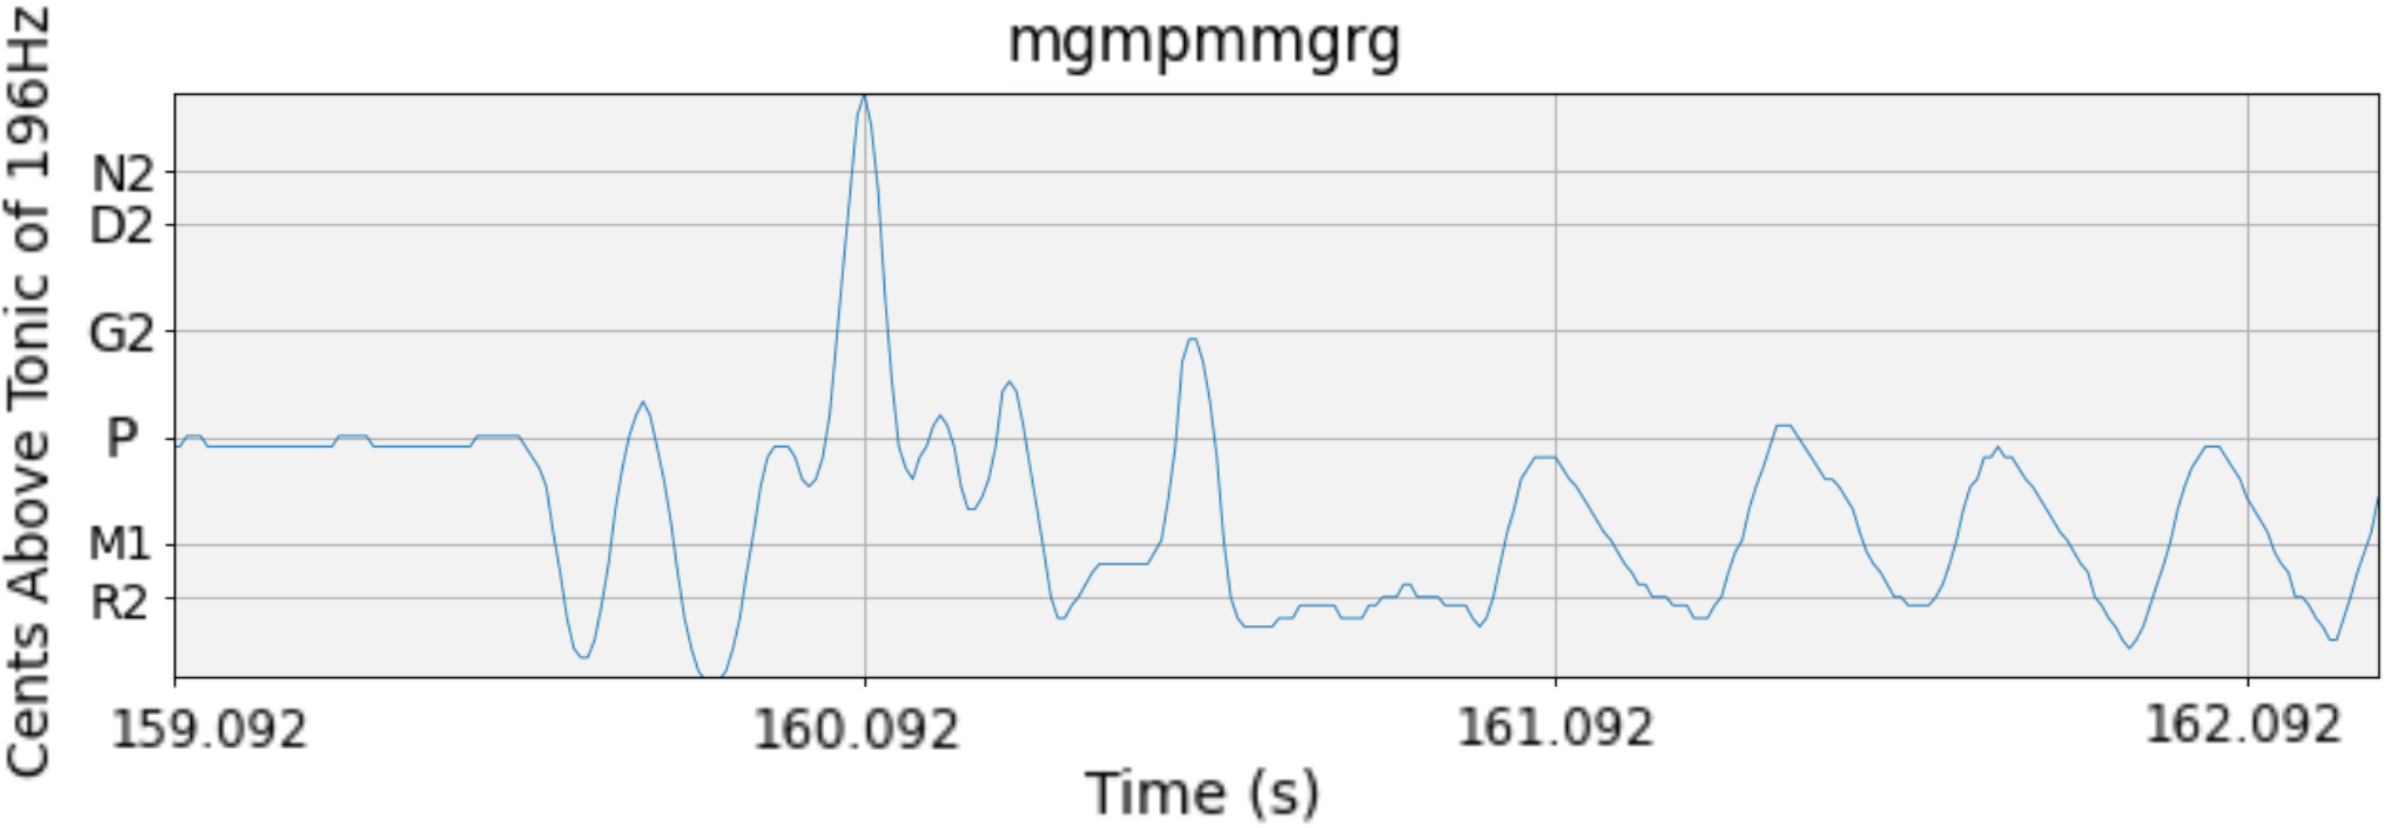
\includegraphics[width=0.9\columnwidth]{ch02_sb/figures/pitch_plot.png}}
    \caption{\textbf{Pitch movement for sañcāra \textit{mgmpmmgrg} from the recording of Koti Janmani in rāga rītigauḷa, sung by the Akkarai Sisters.} It can be seen that the long ga at the end of the phrase is performed as an oscillation between ri and ma, which is typical for this rāga. Plot provided by Thomas Nuttall and Dr. Lara Pearson from the experiments in~\citep{nuttall-sancaras}. Pitch track computed using a FTANet-Carnatic, developed in this thesis (Chapter~\ref{ch04_melody}).}
    \label{fig:ch02:pitch_plot}
\end{figure}




This oscillatory movement is particularly characteristic of the Carnatic style, and can often subsume individual svaras~\citep{pearson-coarticulation}. The surface effect on the melodic line is that it typically has fewer stable pitch regions than many other styles, as seen in Figure~\ref{fig:ch02:pitch_plot}. Such qualities makes it impossible for researchers who are not themselves Carnatic musicians to reliably identify svaras from audio recordings.\footnote{Recent work has attempted to automate this task by creating descriptive transcriptions that assign svara names to key points in the melodic flow~\citep{ranjani-quantized,ranjani-compact,viraraghavan-state_based}. However, such descriptive transcriptions do not necessarily align with the underlying svaras that musicians would use to notate the phrase, which may or may not be a problem, depending on the research question and purpose of the transcription.}

%The heavy use of gamakas, especially oscillations, makes automated transcription of Carnatic music a challenging task. 



\paragraph*{Sañc\={a}ra.}
Another important feature of the style is the structural and expressive significance of motifs and phrases known as sañc\={a}ras, which can be defined as coherent segments of melodic movement that follow the grammar of the rāga~\citep{viswanathan-alapana,pesch-book}. The term sañcāra comes from sanskrit and it means to move.
%The term sañcāra comes from the Sanskrit root सञ्चर्, meaning to move. 
Although occasionally the term might be used to refer to phrases that are particularly characteristic of a r\={a}ga, the more common use of the term is in reference to any melodic segment that is coherent from a Carnatic music perspective. These melodic patterns are the means through which the character of the r\={a}ga is expressed and they form the basis of various improvisatory and compositional formats in the style~\citep{viswanathan-alapana,ishwar-motif_alapana}. 
%
There are no definitive lists of all possible sañcāras in each rāga, rather the body of existing compositions and the living oral tradition of rāga performance act as repositories for that knowledge.\footnote{Sañcāras are the building blocks of Carnatic music, and so there is considerable musicological interest in searching for them. However, as is the case with the related concept of \textit{musical phrase}, there may be ambiguity regarding the borders of the sañcāra: for example, different annotators may segment at different hierarchical levels (for a related discussion in the context of Western popular music, see~\cite{bruderer-perception}).}

\paragraph*{Characteristic phrases or pi\d{d}is.}
These are phrases that can only be found in one rāga, and thus point clearly to that rāga. As explained by the Carnatic musician and musicologist T. Viswanathan, \textit{“each rāga has its own characteristic phrases which appear regularly in compositions, and which are guaranteed to produce instant recognition–-and, if well performed, appreciation–-in the audience”} (\cite{viswanathan-alapana}, p. 38).

%Implications for MIR: Many rāgas will be identifiable from key characteristic motifs (piḍis).

\paragraph*{Tanpura drone.}
The tambūrā creates a consistent and plucked drone, which includes sa (ṣaḍja) and usually pa (pañcama), the perfect fifth above (although in some rāgas, ma might be used as the other tone). Sa is set to the pitch in which the singer/instrumentalist feels most comfortable performing.
The tone ṣaḍja (sa) has a tonic-like effect, where we feel a sense of rest on that tone, and hence it is sometimes referred to by musicologists as the \textit{tonic}, even though no such term exists in Carnatic music.

%Implications for MIR: sa can be placed at any pitch, and usually remains the same throughout a performance. However a few rāgas may be presented in the madhyama śruti, which shifts the position of sa. The fact that sa may be placed at any pitch means that for many MIR processes, pitch needs to be normalized to wherever sa is placed.





\section{Computational melodic analysis of IAM}\label{ch02_sb:sec:computational-carnatic}
%Proof of the research importance given to the computational analysis of Carnatic Music, in addition to an important body of literature focusing on this topic
The computational and corpus-based analysis of \acrshort{IAM} is an important research topic, proof of which are the multiple doctoral dissertations that have been carried out covering \textbf{melodic}~\citep{gulati-thesis,gopala-thesis,ross-thesis}, \textbf{rhythmic}~\citep{ajay-thesis}\footnote{Rhythm is also particularly relevant for both Carnatic and Hindustani as it may facilitate structural and analysis segmentation~\citep{rao-dhrupad}.} and \textbf{structural}~\citep{ranjani-thesis} aspects for the Carnatic and Hindustani styles. Existing works also explore \textbf{timbre} analysis, particularly focusing on percussion instruments like the mridangam and tabla \citep{anantapadmanabhan-mridangam_1,anantapadmanabhan-mridangam_2,rohit-tabla}.
%
%Beyond the Indian context, the CompMusic project has engaged computational studies tailored to other art music traditions, including Turkish-Makam~\citep{senturk-thesis} and Jingju (Beijing Opera) music~citep{gong-thesis,rafa-thesis}. These endeavors underscore the versatility and applicability of computational methodologies across diverse musical cultures.

Nonetheless, the primary emphasis of this dissertation is on melodic analysis. Given the key role of melody in Carnatic music, a comprehensive overview of prior research efforts in this domain is now provided, setting the foundation for the contributions of this work.
%
%Including the presence of works also focusing on \textbf{timbre} analysis~\citep{anantapadmanabhan-mridangam_1,anantapadmanabhan-mridangam_2,rohit-tabla}, these are the four music dimensions we use as reference to divide the literature on computational analysis of the art music traditions from India. In the upcoming Sections we provide an overview of prior research efforts on each of these four dimensions, with an especial emphasis to melodic analysis, which is where this dissertation sets the scope.
%
%\subsection{Melodic analysis of IAM}\label%{ch02_sb:sec:melodic-analysis}
%%%%%%%%%%%% Vocal intonation analysis
The reader is kindly referred to Tables~\ref{tab:survey_1} and \ref{tab:survey_2} for an overview of existing work on computational melodic analysis of Carnatic and Hindustani Music.\footnote{Please note this review is not meant to be fully exhaustive. Instead, this is meant to be an extensive survey that considers impactful research efforts representing different researchers, projects, institutions, providing a faithful overview of the advancements in the field.}



\paragraph*{Tonic identification.} 
Tonic identification is a foundational problem in the computational analysis of Carnatic music, as the tonic \textit{Sa} serves as the reference pitch for the entirety of melodic and harmonic elements. Early approaches utilized heuristic methods, leveraging the presence of the drone (normally played by the tanpura) to estimate the tonic frequency. For instance, techniques based on autocorrelation and spectral analysis~\citep{decheveigne-yin,rao-pitch,salamon-sinusoid} have been employed to detect the prominent frequencies corresponding to the tonic~\citep{sengupta-tonic,ranjani-tonic,bellur-tonic,salamon-tonic}.

Subsequent methods incorporated statistical models and machine learning algorithms to improve accuracy, especially enhancing robustness to polyphonic contexts where multiple instruments and vocals are present~\citep{gulati-tonic_old,gulati-tonic,aiswarya-tonic}. These models analyze pitch histograms and employ classification techniques to discern the tonic amidst complex musical textures. Recent work has explored \acrshort{DL} approaches, utilizing neural networks trained on annotated datasets to identify the tonic~\citep{singh-tonic}. 

As seen in Table~\ref{tab:survey_1}, the entirety of the reviewed approaches rely on pitch-related features, generally extracted using heuristic methods to extract the predominant pitch from music mixtures. Only in the case of \citep{singh-tonic}, a signal processing based harmonic-percussive separation method is used to facilitate the melodic feature processing~\citep{driedge-harmonic_separation}.


\begin{table}[p]
\centering
\footnotesize
\caption{\textbf{Overview of pitch tracking and separation processes in melodic analysis studies;} in this table we cover the following tasks: tonic identification, singing voice analysis and classification, svara transcription and analysis, structure segmentation, and multimodal studies. See other tasks in Table~\ref{tab:survey_2}.}
%Works with no pitch track method explicitly indicated operate on annotated svaras or pitch-independent hand-crafted audio features. Works with no separation model indicated operate on mixture signals, or scores.
\label{tab:survey_1}
\begin{adjustbox}{max width=\textwidth}
\begin{tabular}{l p{2.2cm} p{3.8cm} p{3.1cm}}
\toprule
\textbf{Reference} & \textbf{Method} & \textbf{Pitch Track} & \textbf{Separation} \\
\midrule
\midrule
\multicolumn{4}{l}{\textbf{Tonic identification}} \\
\midrule
\citep{sengupta-tonic} & \textcolor{olive}{Heuristics} & Rao \& Rao (2010) & -- \\
\citep{ranjani-tonic} & \textcolor{olive}{Heuristics} & Autocorrelation & -- \\
\citep{bellur-tonic} & \textcolor{olive}{Heuristics} & YIN & -- \\
\citep{gulati-tonic_old} & \textcolor{olive}{Heuristics}, \textcolor{red}{ML}  & Salamon et al. (2011) & -- \\
\citep{salamon-tonic} & \textcolor{olive}{Heuristics} & Salamon et al. (2011) & -- \\
\citep{bellur-tonic_cepstrum} & \textcolor{olive}{Heuristics} & Custom heuristic & -- \\
\citep{gulati-tonic} & \textcolor{olive}{Heuristics}, \textcolor{red}{ML} & Melodia & -- \\
\citep{singh-tonic} & \textcolor{cyan}{DL} & Klapuri (2006) & Driedger et al. (2014) \\
\citep{aiswarya-tonic} & \textcolor{olive}{Heuristics}, \textcolor{red}{ML} & Camacho et al. (2008) & -- \\
\midrule
\multicolumn{4}{l}{\textbf{Singing voice analysis and classification}} \\
\midrule
\citep{vidwans-classification} & \textcolor{teal}{Stat. modeling} & Rao \& Rao (2010) & -- \\
\citep{koduri-characterization} & \textcolor{teal}{Stat. modeling} & YIN + Melodia & -- \\
\citep{koduri-intonation} & \textcolor{red}{ML} & Melodia & -- \\
\midrule
\multicolumn{4}{l}{\textbf{Melody transcription, descriptive notation, analysis, and generation}} \\
\midrule
\citep{miryala-transcription} & \textcolor{olive}{Heuristics} & Autocorrelation & -- \\
\citep{gulati-landmark} & \textcolor{red}{ML} & Melodia  & -- \\
\citep{gulati-evaluation} & \textcolor{teal}{Stat. modeling} & Melodia + Rao (2010) & -- \\
\citep{ganguli-structures} & \textcolor{red}{ML} & Melodia & -- \\
\citep{senturk-svaras} & \textcolor{teal}{Stat. modeling} & -- & -- \\
\citep{ranjani-quantized} & \textcolor{teal}{Stat. modeling} & Autocorrelation & -- \\
\citep{dhara-transciption} & \textcolor{teal}{Stat. modeling} & Melodia & -- \\
\citep{ranjani-compact} & \textcolor{teal}{Stat. modeling} & Melodia & -- \\
\citep{nuttall-svara} & \textcolor{cyan}{DL} & Plaja-Roglans et al. (2023) & -- \\
\citep{shikarpur-hierarchical} & \textcolor{cyan}{DL} & CREPE & H-Demucs \\
\midrule
\multicolumn{4}{l}{\textbf{Structure analysis and segmentation}} \\
\midrule
\citep{verma-structural} & \textcolor{olive}{Heuristics} & -- & -- \\
\citep{ranjani-structural} & \textcolor{cyan}{DL} & Melodia & -- \\
\midrule
\multicolumn{4}{l}{\textbf{Performance analysis via multimodal studies}} \\
\midrule
\citep{pearson-gesture_sonic} & \textcolor{violet}{Analytical} & Autocorrelation & -- \\
\citep{pearson-coarticulation} & \textcolor{violet}{Analytical} & Autocorrelation & -- \\
\citep{pearson-gesture_coupling} & \textcolor{teal}{Stat. modeling} & Autocorrelation & -- \\
\citep{pearson-landscapes} & \textcolor{teal}{Stat. modeling} & Plaja-Roglans et al. (2023) & -- \\
\citep{nadkarni-exploring} & \textcolor{cyan}{DL} & Autocorrelation & Spleeter (+ ANR) \\
\citep{nadkarni-gesture_motifs} & \textcolor{cyan}{DL} & Autocorrelation & Spleeter (+ ANR) \\
\bottomrule
\end{tabular}
\end{adjustbox}
\vfill\clearpage
\end{table}


\paragraph*{Singing voice analysis and classification.}
Because the singing voice leads the most common format in both Carnatic and Hindustani music,
%–-and is the source for which the most tailored analysis and processing systems exist–-
melodic analysis in Carnatic music strongly relies on the vocal source and melody.
%
Existing work have studied particular singing aspects of the singing voice, attempting to characterize vocal intonation~\citep{koduri-characterization,koduri-intonation} or classification of vocal styles~\citep{vidwans-classification}. These approaches generally operate on statistical features from the pitch contours.


\paragraph*{Melody transcription, descriptive notation, and analysis.}
Melody transcription in Carnatic music involves converting audio recordings into symbolic representations, capturing the sequence of notes (svaras) and in some cases, their expressive nuances. Traditional methods used to rely on heuristic algorithms to map pitch contours into the corresponding svaras~\citep{miryala-transcription}. %often using autocorrelation techniques for pitch detection.
%Statistical modeling approaches 
On the other hand, Hidden Markov Models (HMM) have been employed to model the temporal progression of notes and account for the probabilistic nature of musical transitions~\citep{ranjani-quantized,ranjani-compact}. These models consider the contextual information and typical patterns in Carnatic compositions to enhance transcription accuracy. 
%
Data-driven techniques have also been used to analyse the pitch contours and identify structures that enable the detection of theoretical notes~\citep{gulati-landmark,ganguli-structures}.
%
More recently, the advent of \acrshort{DL} have enabled the development of more sophisticated systems that can learn complex representations of musical features, enabling more accurate transcription of intricate melodic ornamentations characteristic of Carnatic music~\citep{nuttall-svara}.


\paragraph*{Structure analysis and segmentation.}
Understanding the structural elements of Carnatic compositions, such as sections, motifs, and transitions, is crucial for comprehensive music analysis. Initial studies employed heuristic methods to segment compositions based on changes in pitch, rhythm, or timbre, identifying boundaries between different sections \citep{verma-structural}. Statistical models have been utilized to analyze patterns and repetitions within compositions, aiding in the identification of structural components. Recent research has incorporated deep learning techniques, training models on annotated datasets to automatically detect and segment structural elements in performances \citep{ranjani-structural}. These approaches leverage the ability of neural networks to capture hierarchical and temporal dependencies in music, facilitating more nuanced and accurate structural analysis.

\paragraph*{Performance analysis via multimodal studies.} Music is not only an auditory experience; existing research have shown that the visual and kinetic aspects play a key role for comprehensive music analysis~\citep{clarke-motion,godoy-motor_mimetic,eitan-multimodal,pearson-coarticulation,sanidha-multimodal}. Along similar lines, analytical studies including interdisciplinary collaborations between musicians, musicologists, and engineers have shed light on how gesture relates to the vocal melody and characteristic melodic patterns~\citep{pearson-gesture_sonic,pearson-gesture_coupling,pearson-landscapes}. This phenomenon has been thoerized using the concept of \textit{coarticulation} by Dr. Lara Pearson~\citep{pearson-coarticulation}. 


More recently, further efforts have been done to leverage \acrshort{DL} systems to explore the correspondence between gesture and vocal motifs~\citep{nadkarni-exploring}, and subsequently to characterize melodies via kinetic features~\citep{nadkarni-gesture_motifs}. A given set of r\={a}gas have been also classified using a combination of audio and video features, fusing these within the network. An ablation study shows the positive impact of video features, however, audio information in the form of pitch tracks is still essential~\citep{clayton-raga_classification}.



\paragraph*{Melodic pattern discovery and characterization.}
The recognition of melodic patterns is a core aspect of the melodic analysis of \acrshort{IAM}, as note ornaments play a central role in the performance and characterization of rāgas. These ornaments are typically repeated, with subtle variations, along the performance, contributing to the identification of rāgas~\citep{kassebaum-karnatak} and compositions.
%but also of compositions, and even artists.
Melodic pattern discovery for \acrshort{IAM} is therefore an important problem. Most of the proposed approaches build on top of time-series of pitch~\citep{ishwar-motif_alapana,rao-motifs,gulati-mining,gulati-motifs_communities,nuttall-matrix}. In fact, \citep{velankar-pattern_pitch} reviews the melodic recognition task in Carnatic music and concludes that using pitch contours is potentially the best approach. On the same line, a musically-relevant statistical analysis of melodic patterns is proposed in~\citep{viraraghavan-statistical}, aiming at providing a more handy representation of this important aspect for \acrshort{IAM}.

Variation of concurrent melodic patterns is studied in \citep{ganguli-motifs}, relying on pitch contours extracted using \citep{rao-pitch}, which estimates the vocal melody in polyphonic audio by grouping sinusoidal partials based on harmonicity (for more detail see Section~\ref{sec:ch02_pitch_iam}).
%. It leverages the spectral and temporal characteristics of the singing voice to distinguish vocal harmonics from accompaniment, applying temporal smoothness constraints to reduce octave errors. The algorithm computes vocal intensity by measuring the energy of vocal harmonics at each time step. A subsequent enhancement introduced tunable parameters informed by contextual cues such as singer gender and expected pitch variation, improving tracking accuracy in diverse musical settings~\citep{rao-pitch_postprocessing}.
%
More recently, the potential of \acrshort{DL} for melodic pattern discovery has been explored by relying on the learnt pitch features from a complex autoencoder~\citep{nuttall-sancaras}.
%and an attention-based vocal pitch extraction model developed within the context of this dissertation
%Multiple design choices of this entire process are informed by particular Carnatic characteristics. 


%\begin{table}[p]
%\centering
%\caption{Overview of Raga Recognition Approaches.}
%\label{tab:raga_overview}
%\begin{adjustbox}{max width=\textwidth}
%\begin{tabular}{l p{6.5cm} p{3cm} p{2.5cm}}
%\toprule
%Reference & Approach & Pitch Track & Separation \\
%\midrule
%(Pandey et al., 2003) & HMM applied to \textcolor{olive}{Heuristics}-based note transcription & -- & -- \\  % and Pakad matching
%(Chordia et al., 2007) & Distance-based classification using pitch class distribution & Harmonic Product Spectrum (HPS) & -- \\
%(Belle et al., 2009) & Pitch-class distribution & \textcolor{green}{Rao \& Rao, 2010} & -- \\
%(Shetty et al., 2009) & Rule-based svara scale matching & Autocorrelation & -- \\
%(Sridhar et al., 2009) & Manual pattern matching on svara tables per artist & -- & \citep{zhang-separation} \\
%(Bhattacharjee et al., 2011) & Graph-based transition modeling on manual annotated svaras & -- \\
%(Koduri et al., 2011) & \textbf{revise} Analysis of note segmentation and pitch class histogram & \textcolor{green}{Rao \& Rao, 2010} & -- \\
%(Koduri et al., 2012) & K-NN classification on pitch histograms & YIN + Melodia hybrid & -- \\
%(Dighe et al., 2013) & Heuristic classifier using svara histogram \textbf{how are svaras computed?} & -- & -- \\ %done
%(Kumar et al., 2014) & SVM on pitch class profile and n-gram histogram & Melodia & -- \\
%(Gulati et al., 2016a) & \textbf{todo} & Melodia & -- \\
%(Gulati et al., 2016b) & \textbf{revise} HMM/CRF models on phrase-level features & Melodia + silence removal & -- \\
%%%%%(Belle et al., 2016) & Distance-based classification using pitch class distribution and manually validated contours & \textcolor{green}{Rao \& Rao, 2010} & -- \\
%(Ross et al., 2017) & BiLSTM + K-means clustering on note embeddings & Dataset of annotated svaras & -- \\ %done
%(Anand et al., 2019) & CNN applied to chromogram features & Melodia & -- \\
%(Chowdhuri et al., 2019) & \textbf{revise} CNN + RNN models on chromagrams & \textbf{revise} Indirect (via chroma) & -- \\
%(Madhusudhan et al., 2019) & LSTM trained on features from svara sequences & Parselmouth & \citep{drossos2-mad_twinnet} \\ %done
%(Shah et al., 2021) & CNN + LSTM applied to raw spectrograms & -- & Spleeter \\
%%%(Shikarpur et al., 2021) & CNN applied to pitch-based features extracted via Parselmouth & Parselmouth & 4-stem Spleeter  \\ %mode switching not raga recognition!
%(Vasudevan et al., 2021) & Hybrid classifier and clustering system on pitch values & Peak-picking from framed FFT & -- \\ %done
%(Clayton et al., 2022) & Classifier ensemble on multimodal (visual+audio) features & Parselmouth & 4-stem Spleeter \\ %done
%(Vishnu et al., 2022) & LSTM model using MFCC & -- & -- \\ %done
%(John et al., 2020) & CNN applied to pitch features & Parselmouth & 5-stem Spleeter \\ %done,    + denoise
%(Basu et al., 2023) & Two stage \acrshort{\textcolor{cyan}{DL}} model on MFCC & -- & -- \\  %done
%(Jayanthi et al., 2025) & BiLSTM-XGBoost on spectral features \textbf{expand whose?} & -- & -- \\  %done
%\bottomrule
%\end{tabular}
%\end{adjustbox}
%\end{table}


\begin{table}[p]
\centering
\footnotesize
\caption{\textbf{Overview of pitch tracking and separation processes in melodic analysis studies;} in this table we cover melodic pattern discovery and r\={a}ga recognition and analysis. See other tasks in Table~\ref{tab:survey_1}.}
%Works with no pitch track method explicitly indicated operate on annotated svaras or other hand-crafted audio features such as spectrograms of MFCC. Works with no separation model indicated operate on mixture signals, or scores.
\label{tab:survey_2}
\begin{adjustbox}{max width=\textwidth}
\begin{tabular}{l p{2.2cm} p{3.8cm} p{2.7cm}}
\toprule
\textbf{Reference} & \textbf{Method} & \textbf{Pitch Track} & \textbf{Separation} \\
\midrule
\multicolumn{4}{l}{\textbf{Melodic pattern discovery and characterization}} \\
\midrule
\citep{ross-detection} & \textcolor{olive}{Heuristics} & Rao \& Rao (2010) & -- \\
\citep{ross-motifs} & \textcolor{olive}{Heuristics} & Rao \& Rao (2010) & -- \\
\citep{ishwar-motif_alapana} & \textcolor{teal}{Stat. modeling} & Melodia & -- \\
\citep{dutta-motifs} & \textcolor{olive}{Heuristics} & Melodia & -- \\
\citep{gulati-mining} & \textcolor{red}{ML} & Melodia & -- \\
\citep{rao-motifs} & \textcolor{red}{ML} & Melodia + Rao (2010) & -- \\
\citep{ganguli-structures} & \textcolor{red}{ML} & Melodia & -- \\
\citep{gulati-motifs_communities} & \textcolor{red}{ML} & Melodia & -- \\
\citep{ganguli-melodic_shape} & \textcolor{olive}{Heuristics} & Rao \& Rao (2010) & -- \\
\citep{viraraghavan-statistical} & \textcolor{teal}{Stat. modeling} & Melodia & -- \\
\citep{velankar-pattern_pitch} & \textcolor{teal}{Stat. modeling} & (Survey and comparison) & -- \\
\citep{viraraghavan-precision} & \textcolor{teal}{Stat. modeling} & Melodia & -- \\
\citep{viraraghavan-state_based} & \textcolor{teal}{Stat. modeling} & Melodia & -- \\
\citep{velankar-pattern} & \textcolor{olive}{Heuristics} & Autocorrelation & Zhang et al. (2005) \\
\citep{ganguli-motifs} & \textcolor{teal}{Stat. modeling} & Melodia & -- \\
\citep{nuttall-matrix} & \textcolor{olive}{Heuristics} & Melodia & Spleeter \\
\citep{nuttall-sancaras} & \textcolor{cyan}{DL} & Plaja-Roglans et al. (2023) & -- \\
\midrule
\multicolumn{4}{l}{\textbf{R\={a}ga recognition and r\={a}ga performance analysis}} \\
\midrule
\citep{pandey-tansen} & \textcolor{olive}{Heuristics} & Autocorrelation & -- \\
\citep{chordia-raga} & \textcolor{red}{ML} & Harmonic Product Spec. & -- \\
\citep{belle-raga} & \textcolor{red}{ML} & Rao \& Rao (2010) & -- \\
\citep{shetty-raga} & \textcolor{olive}{Heuristics} & Autocorrelation & -- \\
\citep{sridhar-raga} & \textcolor{olive}{Heuristics} & Harmonic Product Spec. & Zhang et al. (2005) \\
\citep{bhattacharjee-raga_transition} & \textcolor{olive}{Heuristics} & -- & -- \\
\citep{koduri-survey} & \textcolor{red}{ML} & Rao \& Rao (2010) & -- \\
\citep{koduri-raga} & \textcolor{red}{ML} & YIN + Melodia & -- \\
\citep{dighe-swara_raga} & \textcolor{olive}{Heuristics} & -- & -- \\
\citep{kumar-raga} & \textcolor{red}{ML} & Melodia & -- \\
\citep{ganguli-ungrammatical}  & \textcolor{teal}{Stat. modeling} & Rao \& Rao (2010) & -- \\
\citep{gulati-time_delayed} & \textcolor{red}{ML} & Melodia & -- \\
\citep{gulati-phrase_raga} & \textcolor{red}{ML} & Melodia & -- \\
\citep{ross-raga_similarity} & \textcolor{cyan}{DL} & -- & -- \\
\citep{ganguli-distributional} & \textcolor{teal}{Stat. modeling} & Rao \& Rao (2010) & - \\
\citep{anand-raga} & \textcolor{cyan}{DL} & Melodia & -- \\
\citep{chowdhuri-raga} & \textcolor{cyan}{DL} & -- & -- \\
\citep{madhusudhan-deepsrgm} & \textcolor{cyan}{DL} & Autocorrelation & MaD-TwinNet \\
\citep{john-carnatic_classification} & \textcolor{cyan}{DL} & Autocorrelation & Spleeter \\
\citep{shah-raga_recognition} & \textcolor{cyan}{DL} & -- & Spleeter \\
\citep{shikarpur-raga_classification} & \textcolor{teal}{Stat. modeling} & Autocorrelation & Spleeter \\ %mode switching not raga recognition!
\citep{vasudevan-hybrid_raga} & \textcolor{red}{ML} & Custom heuristic & -- \\
\citep{clayton-raga_classification} & \textcolor{cyan}{DL} & Autocorrelation & Spleeter \\
\citep{vishnu-lstm_raga} & \textcolor{cyan}{DL} & -- & -- \\
\citep{basu-raga} & \textcolor{cyan}{DL} & -- & -- \\
\citep{jayanthi-raga} & \textcolor{cyan}{DL} & -- & -- \\
\citep{jayanthi-raga} & \textcolor{cyan}{DL} & -- & -- \\
\citep{roychowdhury-raga} & \textcolor{cyan}{DL} & Autocorrelation & Spleeter \\
\bottomrule
\end{tabular}
\end{adjustbox}
\vfill\clearpage
\end{table}



\paragraph*{Rāga recognition and rāga performance analysis}
Automatic rāga recognition is a pivotal task in the computational analysis of \acrshort{IAM}. It facilitates music understanding, archival, and retrieval. Over the years, methodologies have evolved from heuristic approaches to advanced deep learning models. This section provides an overview of these methodologies, emphasizing the features utilized and their respective efficacies. 


Early approaches to rāga recognition predominantly relied on heuristic methods, leveraging melodic cues to model musical structures. These methods often utilized pitch class distributions (PCD) derived from pitch contours obtained through algorithms such as the Harmonic Product Spectrum (HPS) and YIN~\citep{chordia-raga,belle-raga,rao-pitch}. The extracted pitch information was typically folded into a single octave and quantized to create histograms representing the distribution of pitch classes. %, serving as features for classification.

Subsequent methods incorporated statistical models to enhance recognition accuracy. For instance, Support Vector Machines (SVM) and k-Nearest Neighbors (k-NN) classifiers were trained on features like pitch class profiles and n-gram histograms derived from pitch contours extracted using algorithms like Melodia and YIN~\citep{decheveigne-yin,koduri-raga,salamon-melodia,kumar-raga}. Additionally, tradition-specific hand-crafted features~\citep{bhattacharjee-raga_transition,gulati-motifs_communities} and distributional representations of rāga grammar~\citep{ganguli-distributional} were employed to identify and relate rāgas.

Recent advancements for rāga recognition have seen the use of \acrshort{DL} techniques, particularly Convolutional Neural Networks (CNN) and Recurrent Neural Networks (RNN). These models can leverage features such as chromagrams and mel-frequency cepstral coefficients (MFCC)~\citep{chowdhuri-raga,shah-raga_recognition}. However, on the other hand, others yet utilize pitch contours extracted via algorithms like \citep{salamon-melodia} or traditional autocorrelation as inputs to RNN or Long Short-Term Memory~(LSTM) networks~\citep{anand-raga,madhusudhan-deepsrgm}. LSTM in particular have been shown effective in capturing sequential information inherent in musical data, making them suitable for modeling the temporal dynamics of rāgas~\citep{madhusudhan-deepsrgm,vishnu-lstm_raga}. Other recent efforts involve using LSTM-based networks to learn note embeddings from manual svara annotations \citep{ross-raga_similarity}. 


\acrshort{DL} models for rāga recognition have been extended to process multimodal data, fusing hand movements and pitch curves~\citep{clayton-raga_classification,roychowdhury-raga}. While ablation studies indicate the tangible impact of the visual modality, time-aligned pitch curves remain essential for competitive performance. These latter studies rely on a fully-implemented and documented pipeline to clean the raw recordings and compute the features, indicating again the importance of automated data processing techniques for the computational analysis of, in this case, Hindustani music.\footnote{https://github.com/DAP-Lab/hindustani\_raga\_dataset\_processing}

Interestingly, \acrshort{IAM}-driven embeddings of rāga networks, created by establishing connections between lists of rāgas per concert, may be used to develop a recommender system to provide insights for preparing live performances based on the exhaustive organization of rāgas in real concerts~\citep{bagavathi-ragamai}.



%\textbf{Limited Datasets}: The scarcity of large, annotated datasets hampers the training and evaluation of robust models.
%\textbf{Pitch Extraction Errors}: The simultaneous performance of multiple instruments and vocals complicates pitch extraction, leading to octave errors and other inaccuracies. Continuous pitch tracking is necessary, and algorithms like Melodia have been observed to produce fewer errors, as verified through re-synthesis \citep{gulati-motifs_communities}.
%\textbf{Manual Tonic Detection}: Accurate tonic identification is crucial, yet often requires manual intervention, affecting scalability.
%\textbf{Assumptions in Algorithms}: Various methods make assumptions regarding parameters such as the number of swaras, time length, and monophonic nature, which may not hold across diverse musical contexts.
%\textbf{Representation of Ornamentations}: Including ornamentation regions in pitch-class distributions has not significantly improved recognition. Gamakas play an essential role in characterizing rāgas, and their effective exploitation necessitates representing their temporal characteristics, such as actual pitch variation over time. First-order distributions that discard time sequence information are inadequate for this task.





%DL models have been also used for capturing transposition-invariant features for repeated pattern or section identification~\citep{lattner-cae}. Similarly, data summarizations for similarity search may be also achieved through DL models~\citep{wang-embeddings_patterns}. These approaches present relevant for melodic pattern discovery, which is crucial for the computational analysis of Carnatic and Hindustani Music. In fact, the features learnt by the model in~\citep{lattner-cae} have shown promising performance for the said task in a Carnatic scenario~\citep{nuttall-sancaras}

%As per learnt features for IAM signals, \citep{shah-raga_recognition} uses a Convolutional Neural Network (CNN) to extract a feature vector from a pre-processed input signal, and then an LSTM detects sequences in the extracted feature vector. Again, the features extracted using a complex autoencoder provide improved performance for the task of melodic pattern discovery in a Carnatic context~\citep{nuttall-sancaras}. 

%Despite the fact that the reviewed feature extraction strategies present useful for IAM-relevant downstream tasks -- in the majority of the cases providing state-of-the-art results -- to the best of our knowledge no other attempts to learn representations from IAM signals are available. We note the notable use of LSTM networks for rāga recognition, being this approach the most used for this task while reinforcing the relevance of patterns for IAM. We also observe that the research on learning representations and embedding relevant metadata for IAM is scarce, while successful results on attempts for both topics are reported.

% However, challenges persist, including the accurate extraction of pitch in polyphonic contexts, the need for extensive annotated datasets, and the variability inherent in musical performances. Future research directions may focus on developing robust pitch extraction algorithms capable of handling complex musical textures and exploring unsupervised learning techniques to mitigate the reliance on large labeled datasets.




\section{Predominant and vocal melody extraction}\label{ch02_sb:sec:pitch-extraction}
Section~\ref{ch02_sb:sec:computational-carnatic} highlights the importance of time-series of predominant or vocal pitch for the computational analysis Carnatic music. Pitch contours serve as relevant information for computational musicology studies but also as input feature for other analysis tasks such as tonic identification~\citep{salamon-tonic} or svara transcription~\citep{dhara-transciption}. 
%
Even with the advent of \acrshort{DL} systems which learn patterns directly from the raw data, pitch contours remain a crucial feature in the analysis of Carnatic music, some examples being~\citep{anand-raga,john-carnatic_classification,nuttall-sancaras}. 
%
%The task is predominant or vocal melody extraction can be formally defined as the automatic prediction of the pitch values, at small frames, sung by the lead singer of a musical piece.

%We also observe that pitch contours are also~\citep{john-carnatic_classification,singh-tonic}, while music section segmentation in an \acrshort{IAM} context can also be approached using pitch time-series~\citep{ranjani-structural}.

%
While distributing individual stems for Carnatic music is rare, there is a scarcity of Carnatic-tailored stem separation systems (further discussed in Section~\ref{ch02_sb:sec:music-source-separation}). Thus, researchers are compelled to estimate the pitch contours directly from polyphonic mixture signals. Moreover, the heterogeneity in melodic textures, the tuned percussion, and the rich drone make the predominant estimation of pitch contours a particularly complex task, which is even further complicated if we are interested in the melody performed by a single source.
%


\subsection{Background and current trends}
The task of predominant pitch estimation should not be confused with pitch tracking–-estimating the fundamental frequency of an isolated, monophonic source–-or multi-pitch estimation–-detecting all existing pitch curves in a polyphonic signal~\citep{bittner-thesis}. As already motivated, in this dissertation we focus on vocal pitch estimation, which
%is a class of predominant pitch extraction which
targets solely the melody corresponding to the singing voice. In contrast to melody \textit{transcription}, which targets discrete notes, \acrshort{VME} is aimed at estimating, in very small frames, frequency values.


\paragraph{Salience-based methods.} These class of main melody estimation methods first compute a salience function, often via harmonic summation or spectral peak filtering on a time–frequency representation (e.g. \acrfull{STFT} or constant-Q). Then, the pitch contours are selected using continuity and octave-error penalties, and voicing detection is applied via thresholding or simple statistical models~\citep{goto-f0,poliner-transcription,rao-pitch,salamon-melodia}.


\paragraph*{Modelling-based approaches.} This class of systems explicitly decomposes the audio into a lead melodic source and accompaniment using structured models. Earlier, NMF-assisted separation was introduced to the problem, pioneering the combined extraction/separation paradigm~\citep{durrieu-singer}.
%
Subsequently, \citep{durrieu-source_filter} introduced a source/filter model in which the singing voice is modeled as a harmonic excitation shaped by a timbral filter. Parameters are learned in an unsupervised maximum-likelihood framework, and melodic $f_0$ contours are extracted via Viterbi smoothing or threshold-based voicing decisions. The approach is extended to provide a mid-level representation\footnote{A mid-level representation in audio signal processing captures perceptually meaningful features—such as pitch, rhythm, or harmony–-that are more abstract than raw waveform data but more interpretable than symbolic notation. These representations bridge the gap between low-level features like the \acrshort{STFT} and high-level semantic information, facilitating tasks like melody extraction and music retrieval.} to support source separation via Wiener filtering \citep{durrieu-musically}. Similarly, \citep{fuentes-probabilistic} proposed a probabilistic model that utilizes the Constant-Q Transform to model this problem.




%\paragraph*{Heuristic methods.} For many years, predominant pitch estimation was approached using heuristic methods, which generally rely on the harmonicity of the source to extract the corresponding pitch curve, some well-known examples being~\citep{durrieu-source_filter,rao-pitch,salamon-melodia}. These methods showed enhanced robustness to the presence of accompaniment, positioning them as popular alternatives to methods such as autocorrelation~\citep{rabiner-autocorrelation}, YIN~\citep{decheveigne-yin}, SWIPE~\citep{camacho-sawtooth} PYIN~\citep{mauch-pyin}, which assume a monophonic source as input. Moreover, these methods have been key for music domains for which open annotated predominant melody datasets are not available, offering an alternative solution to the emerging \acrshort{DL} approaches that were showing promising performance and efficiency~\citep{bittner-contour_class,bittner-deep_salience}.


%However, predominant and vocal pitch estimation are complex tasks for which 
\paragraph*{\acrshort{DL}-based approaches.} In the very recent years, cutting-edge advances for this task have been proposed~\citep{bittner-deep_salience,jia-tandem_filter,su-patched_cnn,hsieh-encoder_decoder,dong-residual_network,kum-recurrent_network,kum-teacher_student,yu-ftanet,yu-MCSSME,saxena-interactive_extraction,yu-transformer_pitch,hu-singing} mostly relying on late \acrshort{DL} techniques. This non-exhaustive list reflects the persistent interest of the community to refine the source-specific pitch estimation performance, suggesting also that the task is not solved yet.

DL models may be trained to focus on a particular source, 
%Building on top of the Combined Frequency and Periodicity (CFP) features~\citep{su-cfp},
the most common target being the vocal melody~\citep{chou-hybrid_network,kum-teacher_student,yu-ftanet}. This represents an important advancement for \acrshort{IAM}, in which the singing voice plays a key role. 
%
However, in the context of Carnatic music, the presence of strongly overlapping melodic instruments and the idiosyncratic vocal practises add another layer of complexity. That hinders the generalization of existing \acrshort{DL} systems which are generally trained on vocal melody datasets mainly including commercial Western music data~\citep{hsu-mir1k,bittner-medleydb}. For more information please see Section~\ref{ch03_data:sec:melody-datasets} in Chapter~\ref{ch03_data}.
%and therefore may not present proper generalization to out-of-domain repertoires such as Carnatic and Hindustani.
%
%To our best knowledge, ground-truth pitch datasets for the said traditions are not available to date.



\subsection{Melody evaluation metrics}
\label{sec:evaluation_metrics}
A set of comprehensive metrics for melody prediction are designed in \citep{bittner-eval}. These metrics break down the accuracy of the model so the prediction is evaluated from different scopes. Specifically, we have 5 different metrics: \textbf{VR} (Voicing Recall), \textbf{VFA} (Voicing False Alarm), \textbf{RPA} (Raw Pitch Accuracy), \textbf{RCA} (Raw Chroma Accuracy), \textbf{OA} (Overall Accuracy).  
%Let us introduce the nomenclature to mathematically define these metrics. 
Let $n$ be the sample index along the pitch curve. The reference elements are denoted as $f_{n}$ for the frequency values–-represented in Hertz, shortened as Hz–-and $v_{n}$ the reference voicing value (binary). On the other hand, the estimated frequency values are referred as $\hat{f}_{n}$ and the estimated voicing as $\hat{v}_{n}$. We can define the considered melody metrics as:

\begin{itemize}
    \item \textbf{VR} is the rate of frames labeled as belonging to the reference melody that are estimated as actual melody frames.
    \begin{equation}
        \text{VR} = \frac{\sum_{n=0}^{N-1}\hat{v}_nv_n} {\sum_{n=0}^{N-1}v_n}
    \end{equation}
    \item \textbf{VFA} is the rate of frames labeled as not belonging to the target melody that are estimated as actual melody frames. Thus, the lower the better.
    \begin{equation}
        \text{VR} = \frac{\sum_{n=0}^{N-1}\hat{v}_n(1 - v_n)} {\sum_{n=0}^{N-1}(1 - v_n)}
    \end{equation}
    \item \textbf{RPA} is the rate of frequency values in the estimated melody that coincide with the reference values at the respective frame (allowing a $\lambda$ variation between predicted and known values, normally $\frac{1}{2}$ semitone). %However, as stated in \citep{ishwar-master}, this error tolerance fairly works for Western music but it does not exactly apply in our IAM use case, in which we observe ornament and melodic phrases with a higher resolution given the micro-tonal nature of IAM melodies. \textit{For that reason, we tune the pitch accuracy tolerance by reducing the $\lambda$ to a $\nicefrac{1}{4}$ semitone~\citep{ishwar-master}. During the presentation and discussion of the results we consider both mentioned tolerances for compatibility with state of the art results}.
    \begin{equation}
        \text{RPA} = \frac{\sum_{n=0}^{N-1}v_nT_{f_n, \hat{f}_n}} {\sum_{n=0}^{N-1}v_n},\ \text{where}\ T_{f_n, \hat{f}_n} = \left\{\begin{matrix}
        1\ if \ \left | d_s(\hat{f}_n, f_n)) \right | \leq \lambda \\ 
        0\ if \ \left | d_s(\hat{f}_n, f_n)) \right | >  \lambda
        \end{matrix}\right.
    \end{equation}
    Let us remind that $d_s$ is the deviation in cents between the estimated frequency value and the reference.
    
    \item \textbf{RCA} is the same as RPA but both reference and estimated sequences are mapped into a chroma scale before computing the raw pitch accuracy (consequently we ignore octave errors).
    \begin{equation}
        \text{RCA} = \frac{\sum_{n=0}^{N-1}v_nO_{f_n, \hat{f}_n}} {\sum_{n=0}^{N-1}v_n},\ \text{where}\ O_{f_n, \hat{f}_n} = \left\{\begin{matrix}
        1\ if \ \left | d_o(\hat{f}_n, f_n)) \right | \leq \lambda \\ 
        0\ if \ \left | d_o(\hat{f}_n, f_n)) \right | >  \lambda
        \end{matrix}\right.
    \end{equation}
    In this case, $d_o$ works over the chroma scale and therefore, it ignores octave errors by computing the cent difference over a same octave reference. Therefore, this value will be always higher than RPA. The closer this value to RPA, the less octave errors the algorithm is suffering from. 
    
    \item \textbf{OA} is a weighted combination of the other four metrics. It refers to the rate of melody frames that were correctly estimated by the algorithm, considering also the proper identification of the unvoiced regions.
    \begin{equation}
        OA = \frac{1}{N}\sum_{n=0}^{N-1}v_n\hat{v}_nT_{\hat{f}_n, f_n} + (1-v_n)(1-\hat{v}_n)
    \end{equation}
    
\end{itemize}

The most comfortable and standardized manner to compute these metrics is using the \texttt{mir\_eval} Python library.\footnote{\url{https://craffel.github.io/mir\_eval/}}

Nonetheless, predicted pitch accuracy can also be evaluated using the logarithmic absolute frequency error (log-$f_0$ error). This metric provides a stricter and more perceptually meaningful measure of algorithm performance.


\subsection{Predominant pitch extraction in the context of IAM}\label{sec:ch02_pitch_iam}


Referring back to Tables~\ref{tab:survey_1} and \ref{tab:survey_2}, the most recurrently used predominant pitch estimation systems found in the literature survey are the autocorrelation method via PRAAT~\citep{boersma-praat}, the method of \citep{rao-pitch}, and Melodia~\citep{salamon-melodia}, all based on heuristics. 
%
%The scarcity of pitch-annotated datasets for \acrshort{IAM} is preventing the adaptation of \acrshort{DL}-based systems to the Carnatic domain. The closest match is the work of \citep{saxena-interactive_extraction}, which presents a meta-learning based adaptation attempt including an experiment for Hindustani music. %As seen in Tables~\ref{tab:survey_1} and \ref{tab:survey_2}, the computational analysis of Carnatic music rely on the algorithms listed in Table~\ref{tab:pitch-estimation}, being, to the best of our knowledge, the work done in this dissertation~\citep{plaja-pitch} represents the only \acrshort{DL} vocal pitch estimation system that is optimized to operate on Carantic music mixtures.  

\paragraph*{Autocorrelation method~\citep{boersma-praat}.}

It is a widely used method, especially effective for voiced regions of solo speech and singing. It relies on identifying the dominant periodicity (lag) in a short-time window of the signal. The normalized autocorrelation function is defined as:
\begin{equation}
    r_{xx}(\tau) = \frac{\sum_{n=0}^{N-1-\tau} x_w[n] \cdot x_w[n + \tau]}{\sum_{n=0}^{N-1-\tau} w[n] \cdot w[n + \tau]},
\end{equation}

where $x_w[n] = x[n] \cdot w[n]$ is the windowed signal, $w[n]$ is the analysis window (e.g., Hanning), $N$ is the frame length, and $\tau$ the time lag. The estimated fundamental period $\hat{\tau}$ is selected as the lag corresponding to the largest peak in $r_{xx}(\tau)$ within a plausible pitch range (e.g., $75-600$ Hz), excluding $\tau = 0$.
%
Finally, with $f_s$ being the sampling rate, the pitch is computed as:
\begin{equation}
    \hat{F}_0 = \frac{f_s}{\hat{\tau}}
\end{equation}

To smooth the pitch contour, dynamic programming or Viterbi-style tracking are generally applied with cosets that penalize octave errors, large jumps, and voiced/unvoiced switching. A Gaussian low-pass filter before computing $r_{xx}(\tau)$ is often included to improve robustness.

In practise, this method is normally used via PRAAT~\citep{boersma-praat} or parselmouth~\citep{jadoul-parselmouth}–-a Python API for PRAAT.


\begin{table}[t!]
\centering
\footnotesize
\caption{\textbf{Pitch estimation methods used in the computational analysis studies for Carnatic and Hindustani music.} The FTANet-Carnatic model is an output of this thesis, and it is presented in detail in Chapter~\ref{ch04_melody}.}
\label{tab:pitch-estimation}
\begin{tabular}{p{7.4cm} c c}
\toprule
\textbf{Method} & \textbf{for polyph. input} & \textbf{Typology} \\
\midrule
Harmonic Product Spectrum (HPS)~\citep{noll-hps} & \xmark & \textcolor{olive}{Heuristics} \\
Autocorrelation~\citep{rabiner-autocorrelation} & \xmark & \textcolor{olive}{Heuristics} \\
YIN~\citep{decheveigne-yin} & \xmark & \textcolor{olive}{Heuristics} \\
\citep{klapuri-multiple_f0} & (Multiple-$f_0$ est.) & \textcolor{olive}{Heuristics} \\
SWIPE~\citep{camacho-sawtooth} & \xmark & \textcolor{olive}{Heuristics} \\
\citep{rao-pitch} & \cmark & \textcolor{olive}{Heuristics} \\
Melodia~\citep{salamon-melodia} & \cmark & \textcolor{olive}{Heuristics} \\
CREPE~\citep{kim-crepe} & \xmark & \textcolor{cyan}{DL} \\
FTANet-Carnatic~\citep{plaja-pitch}* & \cmark & \textcolor{cyan}{DL} \\
\bottomrule
\end{tabular}
\end{table}




\paragraph*{\citep{rao-pitch}.}
%This method uses harmonicity-based grouping of sinusoidal partials detected in the polyphonic audio to estimate one or more pitch candidates in each frame. Occasionally, the spectral and temporal properties of the singing voice are exploited to discriminate its partials from those of the melodic accompaniment~\citep{rao-pitch_postprocessing}. 
This method performs pitch estimation via harmonic grouping of sinusoidal partials. First, each frame undergoes sinusoidal analysis to detect spectral peaks (or partials) characterized by frequency, amplitude, and phase. These partials are then grouped into harmonic families based on integer-frequency relationships. Each harmonic hypothesis is scored for coherence and amplitude consistency, yielding multiple pitch candidates per frame. To isolate the singing voice, the method includes heuristics based on continuity, spectral energy, and temporal envelope consistency to distinguish vocal partials from accompaniments~\citep{rao-pitch_postprocessing}. A subsequent linking stage creates smooth pitch trajectories by applying dynamic programming with penalties for octave jumps and rapid frequency changes.
 

\paragraph*{Melodia~\citep{salamon-melodia}.}
This algorithm operates by first computing a salience function that highlights prominent frequency components in the audio signal. It then tracks multiple pitch contours over time, which are sequences of pitch candidates that may represent melodic lines. To distinguish the true melody from other contours, Melodia employs heuristic rules based on contour characteristics such as average pitch height, pitch stability, salience, and the presence of vibrato. The raw Melodia pitch contours are often subsequented by post-processing techniques~\citep{gulati-thesis,ganguli-structures} to fill the gaps and solve octave errors.



%To the best of our knowledge, no DL-based data-driven approaches for this task have been proposed to date, and none of the cited models report training or evaluation on Indian Art traditions. In fact, the literature on computational analysis of Carnatic and Hindustani music still relies on heuristic-based approaches \textbf{CITE???}. We hypothesize that one reason for that may be the scarcity of ground-truth vocal pitch annotations for IAM, given that Western-trained models for said task may not be able to fully-generalize to repertoires with a very characteristic melodic framework.

%Efforts towards proposing descriptive representation of pitch time-series are also performed using quantization techniques~\citep{ranjani-quantized,ranjani-compact}. 



%Nonetheless, high-confidence pitch time-series are still the most representative feature for the vocal melody. A broadly used method for pitch extraction in an IAM context is Melodia~\citep{salamon-melodia}, a heuristic approach for predominant pitch extraction from polyphonic music signals.
%
%In the majority of cases in a music distribution scenario, isolated melodic sources are not available. For that reason, an important body of research works have been carried out aiming at extracting the predominant melody from mixture recordings.
%
%The state-of-the-art for said problem is now led by DL approaches~\citep{kum-multi_column,bittner-deep_salience,kum-recurrent_network,hsieh-encoder_decoder}, although no specific architecture type outstands for being the most performing. 



\section{Music source separation}\label{ch02_sb:sec:music-source-separation}
\acrfull{MSS} is the task of automatically separating a mixture into a list of sources or stems~\citep{jansson-unet}. It has received a lot of attention from the \acrshort{MIR} research community given its multiple uses including music production, creation, and practise, but also as a pre-processing step in research pipelines, and even to enhance further retrieval processes~\citep{cortes-enhanced}. Generally, the task of \acrshort{MSS} assumes that a mixture signal $y(t)$ can be modeled as the linear sum of $N$ individual sources:

\begin{equation}\label{eq:mix_mss}
    y(t) = \sum_{n=1}^{N} x_n(t), \quad x_n(t) \text{ is the }n\text{-th source waveform,}
\end{equation}

and the objective is to recover all sources $x_n(t)$ by receiving input mixture $y(t)$. 

\acrshort{MSS} systems ofter leverage time-frequency representations since frequency patterns and structures are useful cues to disentangle musical sources~\citep{jansson-unet}. In this case, mixture $y(t)$ is transformed using the \acrshort{STFT}:
\begin{equation}
    Y(f,\tau) = \mathrm{STFT}\{y(t)\}, \quad \text{ where } Y \in \mathbb{C}^{F \times T},
\end{equation}
and where $\tau$ denotes the time-shift of the analysis window, or frame index.
%i.e.\ the STFT is computed over overlapping frames centered at times $h\tau$, where $h$ is the hop size (frame step).
Next, a separation model estimates $N$ masks $\hat{M}_n(f,\tau)$ which satisfy:
\begin{equation}
    \hat{M}_n(f,\tau) \in [0,1], \quad \sum_{n=1}^N \hat{M}_n(f,\tau) = 1
\end{equation}
Finally, applying the masks to the input mixture yields the estimated $N$ source spectrograms such that:
\begin{equation}
    \hat{S}_n(f,\tau) = \hat{M}_n(f,\tau)\,|Y(f,\tau)|,
\end{equation}
which are inverted back to the time domain. A number of strategies can be used for the synthesis step: reusing the phase information of the input mixture~\citep{jansson-unet}, using a neural vocoder~\citep{kong-hifigan}, and interestingly, another solution is to predict the phase together with the magnitude, including the phase information as additional channels~\citep{choi-cac}.
%
% \[
% \hat{S}_n(f,\tau) = \hat{M}_n(f,\tau)\,|Y(f,\tau)|,
% \]
% followed by inversion:
% \[
% \hat{x}_n(t) = \mathrm{iSTFT}\{\hat{S}_n(f,\tau)\cdot e^{j\angle Y(f,\tau)}\}.
% \]
% The model parameters \(\theta\) are learned by minimizing a supervised loss, e.g.:
% \[
% \mathcal{L}(\theta) = \sum_{n=1}^{N} \left\| \hat{x}_n(t;\theta) - x_n(t) \right\|^2,
% \]
% or alternatively using a spectral-domain loss:
% \[
% \mathcal{L}_{\text{spec}}(\theta) = \sum_{n}\!\sum_{f,\tau} \left|\,|\hat{S}_n(f,\tau)| - |S_n(f,\tau)|\right|,
% \]
% where \(S_n(f,\tau) = \mathrm{STFT}\{x_n(t)\}\) (Enric Gusó et al., 2022) :contentReference[oaicite:1]{index=1}.
%
It is notable to mention that waveform-domain models directly predict signals $\hat{x}_n(t)$ inherently modeling the phase information.

We define the Ideal-Ratio Mask (IRM) as the theoretically best possible frequency mask, composed of values $\in[0, 1]$:
\begin{equation}
    \text{IRM}_{n,f,\tau} = \frac{|S_{n,f,\tau}|}{\sum_{m=1}^{N} |S_{m,f,\tau}|}
\end{equation}
The IRM is important as it is generally used as glass-ceiling reference for the performance of \acrshort{MSS} systems.

Finally, the problem is generally \emph{underdetermined}–-especially in the mono case with \(N>1\)–-necessitating assumptions (e.g., source sparsity, independence) or architectural priors to make the estimation tractable.
%
While the task of source separation for music first focused on extracting the singing voice~\citep{vembu-separation,ozerov-bayesian_sep,rafii-repet}, the models are lately trained on separating a larger set of sources typically \textit{\{vocals, drums, bass, other\}}, the main format in Western commercial music. 


We define \acrfull{SVE} as a sub-task of \acrshort{MSS} which targets the separation of the singing voice stem only~\citep{rafii-overview}. The concept of \textit{extracting a source} it is generally referred to cases where only a mapping from mixture to source is learned, without modeling the rest of sources explicitly, therefore assuming access to pairs of mixture and target sources only. In this case, the inter-source relationships cannot be leveraged~\citep{zhu-instglow}.


%
%Let $y(t)$ now be a musical mixture signal comprising singing voice $x_\mathrm{v}(t)$ and accompaniment $x_\mathrm{a}(t)$:
%\begin{equation}\label{eq:mix_sve}
%    y(t) = x_\mathrm{v}(t) + x_\mathrm{a}(t),
%\end{equation}


\subsection{Background and current trends}
Initial separation attempts for \acrshort{MSS} were done using non-negative matrix factorization~\citep{vembu-separation}, bayesian models~\citep{ozerov-bayesian_sep}, and via identifying repeating patterns in the vocal source~\citep{rafii-repet}. However, similarly to what observed in Section~\ref{ch02_sb:sec:pitch-extraction} for \acrshort{VME}, \acrshort{DL}-based systems have taken over the separation topic showing impressive performance for this complicated problem under relatively limited training data availability. 

\acrshort{MSS} using \acrshort{DL} can be performed on the time~\citep{stoller-waveunet,defossez-demucs_waveform,lluis-end2end}, time-frequency~\citep{jansson-unet,takahashi-d3net}, or a combination of both domains~\citep{defossez-demucs_hybrid,kim-kuielab,yu-danna}. These models are generally trained in a fully-supervised manner, having access to all available sources assuming they sum up to the reference mixture~\citep{zhu-instglow}.


\paragraph*{Waveform-based \acrshort{MSS}.} The literature on \acrshort{MSS} in the waveform domain is generally based on end-to-end encoder/decoder architectures, being the non-causal adaptation of WaveNet~\citep{vandenoord-wavenet,rethage-wavenet_denoising} the only exception. Wave-U-Net~\citep{stoller-waveunet} is an autoencoder inspired by its spectrogram-based counterpart U-Net~\citep{jansson-unet}, while ConvTas-Net~\citep{defossez-demucs_waveform,luo-conv_tasnet} estimates prediction masks in the bottleneck. The leading model is Demucs, now available in two versions v1~\citep{defossez-demucs} and v2~\citep{defossez-demucs_waveform}, which is also an autoencoder with a bidirectional LSTM in the bottleneck. 

However, modeling waveforms is challenging and prone to high-frequency artifacts that penalize the separation performance perceptually and objectively. Moreover, in the context of a problem where frequency structure and patterns are crucial, operating only on waveforms is more opaque to the network. 


\paragraph*{Time-frequency-based \acrshort{MSS}.} Currently the most prominent solution for \acrshort{MSS} is to use time-frequency masks which are multiplied to the input mixture to obtain the target source(s)~\citep{jansson-unet,luo-bsrnn,lu-separation_roformer}. However, these systems are inherently limited by the overlapping patterns and correlation between sources in music, and the need for resynthesizing the predicted spectrograms back to the audio domain.
%
The most common \acrshort{DL} backbone for \acrshort{MSS} are U-Net architectures, first introduced in \citep{ronneberger-unet} for image segmentation, and later ported to the music domain in~\citep{jansson-unet}. U-Net architectures are essentially autoencoders with skip-connections, which directly transfer information from the encoder to the decoder blocks, helping to maintain structure and context.


\paragraph*{Existing challenges and recent developments.} The $4$-stem separation performance has been continuously improving in the recent years due to many advancements such as
%
combining cues from both temporal and spectral domain~\citep{defossez-demucs_hybrid,yu-danna},
%
band-splitting the input spectrogram~\citep{luo-bsrnn,lu-separation_roformer},
%
leveraging transformers to capture and exploit more context~\citep{rouard-transformer_demucs,lu-separation_roformer}, in addition to general \acrshort{DL} development that enable scaled up and more complex networks using less computational resources~\citep{defossez-quantizing}.


\acrshort{DL}-based \acrshort{MSS} systems can also be \textit{conditioned} to tune the separation behaviour or inform the network toward a particular objective. This may include targeting a particular source~\citep{meseguer-unet,petermann-choir}, and/or improving the overall performance~\citep{parekh-motion}. Interestingly, weak information such as vocal magnitude or vocal activity may also be introduced in the separation problem as prior knowledge for better performance~\citep{schulze-weakly}.



\acrshort{MSS} models are normally constrained to a pre-defined set of target sources, which inherently limits the task to a set of domains. Meanwhile, the size and complexity of systems grow faster than the available training data, which is often limited to a few hours. This leads to overfitting and poor generalization to out-of-domain examples. While novel datasets~\citep{pereira-moisesdb,zang-music_restoration} and approaches to consider more sources~\citep{manilow-jukebox,wang-source_fewshot,watcharasupat-agnostic} have been proposed–-in addition to efforts done to compile, including via instrument synthesis, multi-stem datasets for other ensembles~\citep{manilow-slakh,cuesta-cantoria,sarkar-ensembleset}–-competitive \acrshort{MSS} systems remain limited to the Western commercial domain and the \textit{\{vocals, bass, drums, other\}} setup~\citep{richard-audio}.



Given the lack of training data, unsupervised \acrshort{DL} strategies have emerged. \citep{mimilakis-unsupervised} shows that unsupervised autoencoder-based representation learning combined with a sinusoidal synthesis decoder can effectively learn voice-centric features for mask-based separation without supervision. Alternative methods embed differentiable parametric source-filter models within neural networks, enabling training on raw mixtures without isolated sources: first, \citep{schulze-unsupervised} used an external multipitch estimator and heuristic voice-assignment to guide source modeling, and deriving soft masks at inference from reconstructed sources. Subsequently, a fully-differentiable extension of this model has been proposed~\citep{richard-fully}. However, these works operate solely on homonegeous sources–-in this case vocal choirs–-because the parametric source–filter models are designed specifically for similar, harmonically structured vocals, and rely on consistent pitch contours and shared timbral characteristics. These aspects makes them unsuitable for mixtures containing diverse instruments or voice types.


Finally, it is important to note that fully-supervised \acrshort{MSS} systems generally assume the linear sum of Eq.~\ref{eq:mix_mss} to hold true, but this may not always be the case. A first cause for this assumption to fail is a mismatch between the sources that form the mix and individual stems. This in fact constitutes a more realistic real-world mixing scenario, where the final mixture is processed using a number of different non-linear methods (e.g. reverb or dynamic compression). In this case, the separation problem becomes a separation plus restoration task~\citep{zang-music_restoration}. Another cause for Eq.~\ref{eq:mix_mss} not holding true is missing source stems. In this case, %the separation problem becomes weakly-supervised, since 
the joint relation between sources–-which has been shown to contribute to an enhanced separation~\citep{kim-kuielab}–-cannot be exploited. While most of the models introduced in this section can be adapted and trained to extract a single source, this likely adds difficulty as we provide the system with less information~\citep{zhu-instglow}.


\subsection{Music source separation in commercial applications}
\label{ch02_sb:sec:music-source-separation-commercial}
Due to its importance for music production and practise, \acrshort{MSS} has gained a lot of attention from the commercial sector, some well-established examples being Moises,\footnote{\url{https://moises.ai}, please note that part of the work in Chapter~\ref{ch06_sep_gen} of this dissertation has been carried out in an industry internship at Moises.ai, the developers of this application.} AudioShake,\footnote{\url{https://www.audioshake.ai}} GaudioLabs\footnote{\url{https://studio.gaudiolab.io}} and Kits AI.\footnote{\url{https://app.kits.ai/studio}} 


However, these commercial applications are generally based on proprietary models, and therefore, it is not possible to know the exact architecture or training data used. The fact that these applications are not open-sourced, makes it difficult to reproduce the results as companies keep improving their product on a very regular basis.
%or to adapt them to a specific use case.
Moreover, these proprietary applications operate under pricing plans, which restrict their scaled up use in research contexts and again, limit reproducibility for research purposes. For that reason, in this dissertation we focus on open-source models, which are available for the research community to use and adapt, and avoid relying on proprietary models for research pipelines.

As a matter of fact, we were not able to locate a lot of examples of non open-sourced systems in research papers on Carnatic and Hindustani analysis, being \citep{bhake-expressive}, to the best of our knowledge, the only example. However, it is understandable that, for a relatively small amount of data, researchers consider these tools which are normally trained with enormous amount of data and include several post-processing tweaks, aiming at alleviating the domain mismatch that penalize open-sourced systems.





\subsection{Music source separation metrics}\label{sec:source_separation_metrics}

Evaluating music source separation systems typically relies on objective signal-based metrics derived from the BSS Eval framework~\citep{vincent-metrics}. An estimated source $\hat{s}(t)$ is decomposed as:
\begin{equation}
    \hat{s}(t) = s_{\mathrm{target}}(t) + e_{\mathrm{interf}}(t) + e_{\mathrm{noise}}(t) + e_{\mathrm{artif}}(t),
\end{equation}
where $s_{\mathrm{target}}$ is the desired source, $e_{\mathrm{interf}}$ is interference from other sources, $e_{\mathrm{noise}}$ is ambient noise, and $e_{\mathrm{artif}}$ is artifact distortion.

From this decomposition, the classic metrics are defined–-in dB:

\begin{equation}
    \mathrm{SDR} = 10\log_{10} \frac{\|s_{\mathrm{target}}\|^2}{\|e_{\mathrm{interf}} + e_{\mathrm{noise}} + e_{\mathrm{artif}}\|^2}
\end{equation}
\begin{equation}
    \mathrm{SIR} = 10\log_{10} \frac{\|s_{\mathrm{target}}\|^2}{\|e_{\mathrm{interf}}\|^2}
\end{equation}
\begin{equation}
    \mathrm{SAR} = 10\log_{10} \frac{\|s_{\mathrm{target}} + e_{\mathrm{interf}} + e_{\mathrm{noise}}\|^2}{\|e_{\mathrm{artif}}\|^2}
\end{equation}

SDR measures overall distortion, SIR captures interference, and SAR quantifies artifacts~\citep{vincent-metrics}.
%
The original SDR is highly sensitive to scaling, where gain mismatches can distort scores. \citep{roux-sisdr} proposed SI-SDR, which removes this effect by rescaling the estimate:
\begin{equation}
    \mathrm{SI\text{-}SDR} = 10\log_{10} \frac{\|\alpha s_{\mathrm{target}}\|^2}{\|\hat{s} - \alpha s_{\mathrm{target}}\|^2}, \quad \alpha = \frac{\langle \hat{s}, s_{\mathrm{target}} \rangle}{\|s_{\mathrm{target}}\|^2}
\end{equation}

It has been also observed that SDR may correlate poorly with human perception~\citep{cano-evaluation,guso-losses}. 
%suggesting that reporting solely SDR alone may be a limited.
A common practise is to complement the objective measures using perceptual tests with human listeners. These tests are normally based on the MUSHRA framework~\citep{schoeffler-webmushra}. A number of unlabelled separated excerpts corresponding to the outputs of different systems are shown to the participant, who grades them separately in the scale of $1$ to $5$, being $5$ the maximum score. These are known as mean opinion scores (MOS) and are computed as the averaged gradings of all participants.


However, perceptual tests are not reproducible, expensive, and may be subject to limited participant availability or expertise. 
%
Meanwhile, generative audio models are becoming increasingly popular for the separation task given their potential to produce high-fidelity and plausible outputs if properly conditioned or guided~\citep{mariani-msdm}. However, the stochasticity inherent in this systems produces phase mismatches and residual variations that negatively impact waveform-level metrics like SDR and SI-SDR–-especially when the model does not predict waveforms directly but synthesizes audio from latent or spectral representations~\citep{karchkhadze-msdm_ldm}.
%This trade-off is particularly pronounced with diffusion-based or vocoder-style generative systems in source separation or enhancement contexts


%For these reasons, SDR is being less used in prior generative separation work. In the case of LDM, given the added phase reconstruction mismatch introduced by the latent encoder, not even scale-invariant SDR (SI-SDR), present in various generative separation systems~\citep{zhu-instglow,mariani-msdm}, is being used~\citep{karchkhadze-msdm_ldm,chae-mge}.
%
Therefore, alternative audio quality measures are being leveraged to evaluate the fidelity of the separations, some popular examples being log-spectral distance (LSD)~\citep{liu-audioldm} and log mel-spectrogram error~\citep{guso-losses,karchkhadze-msdm_ldm,chae-mge}.
%that have been employed in prior work on latent diffusion for generation~\citep{nistal-diffariff,liu-audioldm} and source separation~\citep{mariani-msdm,karchkhadze-msdm_ldm,chae-mge}: log-spectral distance (LSD)~\citep{liu-audioldm} and log mel-spectrogram L2 error~\citep{guso-losses}.
These metrics are phase-independent and may be more appropriate for generative systems.
%
Although fitting best for music generation and synthesis studies, the quality of the generated signals can be measured without relying on explicitly matching audio pairs using Fréchet Audio Distance (FAD)~\citep{gui-adapting}. Model outputs with higher quality and lesser interferences should report lower FAD. %The FAD is often computed on short chunks. 
%However, in addition to diversity, context is important~\citep{gui-adapting}. Carnatic renditions often feature prolonged improvisational segments, such as \textit{alapana} and \textit{tanam}, which can span several minutes. %Moreover, rhythmic structures (known as \textit{tala}) may unfold over extended time periods. 
%Given the prolonged sections in Carnatic Music renditions, 
%
%For these reasons, we split the samples into $1$-minute chunks.
%in order to enrich the diversity for a more robust metric calculation while representing the aforementioned Carnatic concepts and practices.
%
%We discard the chunks with $>25\%$ of silence, which results in $\approx150$ testing samples. 


Finally, another option is to explicitly evaluate aspects of the generated vocals such as the pitch via log-pitch error~\citep{yi-singing}, or the intelligibility using the perceptual evaluation of speech quality (PESQ)~\citep{pesq} metric. However, it is not clear how well this latter metric characterizes vocal ornaments and how leaked accompaniment affects the scores.


%\subsubsection{Objective evaluation}
%The objective evaluation of generative systems for audio inverse problems is challenging\citep{serra-universe}.
%, and most of the metrics fail to fully correlate with perceptual performance~.
%In MSS, traditional definitions for source-to-distortion ratio (SDR), the standard separation metric, have been reported to often misrepresent the perceptual quality of separations~\citep{cano-evaluation,guso-losses}. Moreover, SDR is significantly penalized by potential subtle differences and phase mismatches commonly present when evaluating fully-generative models.
%
%Consequently, SDR is seeing decreased use in evaluating generative-based separation approaches.


%Objectively evaluating the interference removal capacity of our system is intricate, as the generated vocal components that do not exactly match the target signal may be considered as interferences for certain metrics.


%E-%valuating generative models for inverse problems is a complicated issue, and it is especially pronounced for the task of MSS. While standard dedicated metrics have been reported to often misrepresent the perceptual quality of separations~\citep{cano2016evaluation, guso2022loss}, these metrics are significantly penalized by potential minor differences and phase mismatch between generated separations and target stems. %The stochasticity in the sampling process augments the mismatch.
%Moreover, the reconstruction error of M2L, which is an integral component of our system, exacerbates these discrepancies. 


%

%However, in the context of MSS, perceptual quality and cleanliness are the prioritized aspects for music practitioners and producers.
%establishes also the glass ceiling of the objective performance of our system for particular metrics.

%Having this in mind, we do not find the standard separation metrics useful to quantify the quality of the generated outputs, while speech enhancement metrics are also overly affected by the signal discrepancy and accompaniment interference.
%
%Therefore, existing work relies also on alternative audio quality measures
%that have been employed in prior work on latent diffusion for generation~\citep{nistal-diffariff,liu-audioldm} and source separation~\citep{mariani-msdm,karchkhadze-msdm_ldm,chae-mge}: log-spectral distance (LSD)~\citep{liu-audioldm} and log mel-spectrogram L2 error~\citep{guso-losses}.


%we report the following metrics~\citep{m2l}: \textbf{(1)} SI-SDR (Scale-Invariant Signal-to-Distortion Ratio)~\citep{half_baked}, which is a variant of the standard separation metric which neglects amplitude difference, hence focusing on the structural similarity between separated and reference signals, aligning more closely with human auditory perception, and \textbf{(2)} ViSQOL~\citep{visqol}, which predicts the perceptual quality of audio signals by comparing the generated audio against the reference. 
%\subsubsection{Perceptual assessment}
%With the advent of generative approaches for separation, and the application-based  
%

%since we hypothesize that in our context, a MUSHRA test where participants grade multiple systems in a mean opinion score (MOS) scale may be complicated and prone to inter-user disagreement.
%
%We split the separations into chunks of $\approx15$ seconds, discarding unvoiced regions, and randomly select an instance for each rendition. Using the mixture as reference, we select $6$ examples from the pool, including diversity of music sections and singer gender.

%The participants are shown several unlabeled and randomly ordered pairs of samples of our model against other systems.
%\textit{cold-diff}~\citep{plaja2023carnatic}, the \textit{mixer} model~\citep{wimaga}, and MSDM~\citep{mariani2023multi}. 
%We introduce comparisons between non-generative models to prevent the participants from getting familiar with model-specific artifacts. %The reference mixture or vocals are not shown, aiming at focusing the attention of users on the preference between the shown pair. 








% \vspace{0.5em}
% \noindent\textbf{Time–frequency representation (STFT):}  
% \[
% Y(f,\tau) = \mathrm{STFT}\{y(t)\},\quad S_\mathrm{v}(f,\tau) = \mathrm{STFT}\{x_\mathrm{v}(t)\},\quad S_\mathrm{a}(f,\tau) = \mathrm{STFT}\{x_\mathrm{a}(t)\}.
% \]

% A common strategy estimates a mask \(\hat{M}(f,\tau)\) that highlights singing voice bins:

% \[
% \hat{S}_\mathrm{v}(f,\tau) = \hat{M}(f,\tau)\cdot|Y(f,\tau)|,\quad
% \hat{S}_\mathrm{a}(f,\tau) = [1 - \hat{M}(f,\tau)]\cdot|Y(f,\tau)|.
% \]

% The corresponding time-domain signals are obtained via inverse STFT:

% \[
% \hat{x}_\mathrm{v}(t) = \mathrm{iSTFT}\{\hat{S}_\mathrm{v}(f,\tau)\cdot e^{j\angle Y(f,\tau)}\},\quad
% \hat{x}_\mathrm{a}(t) = \mathrm{iSTFT}\{\hat{S}_\mathrm{a}(f,\tau)\cdot e^{j\angle Y(f,\tau)}\}.
% \]


% \vspace{0.5em}
% \noindent\textbf{Optimization objective:}  
% Train a model \(M_\theta\) (e.g., a DNN) to predict \(\hat{M}\) using supervised loss. For instance, the cross-entropy loss to match an IBM target:

% \[
% \mathcal{L}_\mathrm{CE}(\theta) = -\sum_{f,\tau}\Bigl[ M_\mathrm{IBM}(f,\tau)\log \hat{M}_\theta(f,\tau) + (1 - M_\mathrm{IBM}(f,\tau))\log(1 - \hat{M}_\theta(f,\tau))\Bigr].
% \]

% Alternatively, a waveform-domain loss on reconstructed signals:

% \[
% \mathcal{L}_\mathrm{wave}(\theta) = \| \hat{x}_\mathrm{v}(t; \theta) - x_\mathrm{v}(t)\|_2^2 + \| \hat{x}_\mathrm{a}(t; \theta) - x_\mathrm{a}(t)\|_2^2.
% \]

% Both objectives are commonly used in recent deep-learning based systems :contentReference[oaicite:3]{index=3}.

% ---

% \noindent\textbf{Summary:}  
% Singing voice extraction is defined as estimating \(\hat{x}_\mathrm{v}(t)\) and \(\hat{x}_\mathrm{a}(t)\) from

% \[
% y(t) = x_\mathrm{v}(t) + x_\mathrm{a}(t),
% \]

% by learning a mask \(\hat{M}(f,\tau)\) applied to the mixture spectrum and training either on mask-based cross-entropy or waveform-domain reconstruction losses, achieving separation of vocals from accompaniment.


\subsection{Singing voice extraction in the context of IAM}
Carnatic music is a repertoire that presents several challenges for the task of \acrshort{MSS} and \acrshort{SVE}. To the best of our knowledge, no Carnatic-centered source separation systems are available as of the starting date of the work of this thesis–-not even to separate the singing voice–-compeling researchers to use available pre-trained \acrshort{DL} models~\citep{nuttall-matrix,shah-raga_recognition,clayton-raga_classification}. In the data collections used to train these systems, Carnatic and Hindustani music are very likely not included, since the pre-defined sources do not map to the Carnatic arrangement. Similarly to the case of \acrshort{VME}, these models may not properly generalize to Carnatic audio given the strong, concurrent, and micro-tonal vocal ornaments, in addition to an ubiquitous arrangement featuring prominent melodic instruments; in fact, even the percussion is pitched and harmonically-consistent with the other sources. No detailed study for this problem is present in the literature, while clean multi-stem datasets for Carnatic music are only available in small amounts~\citep{sanidha-multimodal}.\footnote{The dataset of \citep{sanidha-multimodal}, which is further introduced in Section~\ref{ch03_data:sec:separation-datasets}, was published right at the final year of this PhD thesis.}



\subsection{New directions in MSS: generative models}
\label{ch02_sb:sec:future-directions-mss}
Time-frequency masking remains the dominant approach for \acrshort{MSS} due to their strong benchmark performance and interpretability. However, this approach has several limitations: \textbf{(i)} assumptions on sparsity and independence in the time-frequency domain can lead to suboptimal separation quality, especially in complex mixtures with overlapping harmonic content, \textbf{(ii)} the need to reconstruct the phase information from the mixture can introduce artifacts~\citep{defossez-demucs_waveform}, and \textbf{(iii)} the limited availability of large-scale annotated datasets restricts the generalization capabilities of these models, which become prone to overfitting and domain mismatch~\citep{bugler-transfer_separation}.

Despite not being yet a mature area of research, promising results for \acrshort{MSS} and \acrshort{SVE} have been achieved using \acrfull{DDPM}~\citep{mariani-msdm,karchkhadze-msdm_ldm}. These models are trained to generate the target source(s), bypassing the need for explicit masking. % and also generally skipping the phase reconstruction step.
Recent advancements in \acrshort{DDPM} are enabling the development of robust systems that are capable of addressing inverse problems, showing better generalization while achieving competitive audio quality~\citep{serra-universe}. 


In fact, \acrshort{DDPM} are considered a promising future direction for \acrshort{MSS} and \acrshort{SVE} given their flexibility and generalization capabilities~\citep{araki-30years}. This is relevant also for the computational analysis of musical repertoires that do not fall into the Western modern music category, as the generalization capabilities of \acrshort{DDPM} could contribute to a less dramatic performance drop due to domain shift.
% in \acrshort{MSS}.
%
For all these reasons, \acrshort{DDPM} for separation is studied in this thesis. We will first apply their underlying principles in the deterministic regime, but we also explore their generative potential and flexibility for the task of \acrshort{SVE}. The next Section provides a brief introduction to this powerful class of generative models. The technical background of the diffusion backbones leveraged in this thesis are introduced in Chapter~\ref{ch05_sep_nongen}, Section~\ref{ch05_sep_nongen:sec:background} and in Chapter~\ref{ch06_sep_gen}, Section~\ref{ch06_sep_gen:sec:background}.
%\section{Conclusions}
%From the survey of the state-of-the-art we observe several relevant points: 
%\begin{itemize}
    %
%    \itemsep0em
    %
%    \item The Dunya corpora are the main source of data used in computational analysis for IAM signals.
    %
%    \item We note the relevance of the singing voice, concluding that an improved feature extraction on top of vocal data would better assist further musicologically-relevant research for the Carnatic and Hindustani traditions.
    %
%    \item We also note that using deep embeddings or learnt representations in an IAM context has been shown to achieve state-of-the-art results for musicologically-relevant problems. Nonetheless, the body of literature on the said topics is not very large, which may be due to the scarcity of ongoing efforts to focus on the computational analysis of musical repertoires out of the mainstream Western music domain.
    %
%    \item For most of the covered tasks and problems in this literature review chapter, we observe a common issue: there is a domain gap -- i.e. repertoire or tradition gap -- in the field of MIR, caused by the difference in performance of state-of-the-art approaches between Western commercial music and signals out of that class. In this thesis, we aim at contributing to bridge said gap by tailoring the proposed approaches on particular repertoires. 
%\end{itemize}



%\acrfull{SVE}, which involves separating the vocal source from music recording mixtures, has received a lot of attention from the \acrfull{ASP} and \acrfull{MIR} communities in the recent years. This problem can be modeled in the waveform domain~\citep{defossez-demucs,rethage-wavenet_denoising,luo-conv_tasnet}, the frequency domain~\citep{takahashi-d3net,li-sams_net,jansson-unet}, or a combination of both~\citep{defossez-demucs_hybrid,kim-kuielab,yu-danna}. In general, spectrogram-based approaches have been more popular despite having to deal with the problem of the complex phase, usually leading to artifacts or unnaturalness of the separated sources. Within the Music Demixing Challenge (MDX) framed in ISMIR 2021~\citep{dmx-challenge}, diverse submissions achieved state-of-the-art source separation performance,
%on the BSS Eval metrics~\citep{metrics},
%in the majority of cases being multi-branch networks combining features from both time and frequency domains, proposing therefore solutions to account for the problem with the phase. Nonetheless, these models tend to be heavy-weighted and include engineered strategies to improve the predicted outputs.
%

%While the problem of source separation has been shown to be challenging on the waveform domain, promising results have been reported~\citep{rethage-wavenet_denoising, stoller-waveunet, defossez-demucs}, opening the door for the development of models that bypass the problem with the complex phase. However, as the performance improves, the model size and complexity accordingly grow.






\section{Denoising diffusion probabilistic models}\label{ch02_sb:sec:ddpm}
\acrshort{DDPM} are a novel class of generative models theoretically grounded in the non-equilibrium statistical physics that can gradually convert one distribution into another using a Markov chain~\citep{dickstein-thermodynamics}, while learning to perform the reverse process. More concisely, the diffusion forward process converts a signal from a particular data distribution to a simple one (e.g. Gaussian noise) by gradually adding samples of the simple distribution. Subsequently, the model is trained to reverse the noising process to generate samples of the original distribution~\citep{ho-diffusion}. \acrshort{DDPM} have recently emerged as a versatile and high-performance method, outperforming prior approaches for diverse generation tasks~\citep{dhariwal-diffusion}.


In the recent years, numerous improvements have been built on top of the standard diffusion formalization aiming at improving on quality and efficiency. Some of these include, but are not limited to, the use of deterministic perturbation signals~\citep{arpit-cold_diffusion}, the use of compact latent representations as generation targets~\citep{rombach-highresolution}, technical improvements for the diffusion forward~\citep{song-ddim} and sampling processes~\citep{salimans-progressive}, and powerful conditioning and guidance techniques~\citep{serra-universe,zhang-controlnet,bansal-universal_guidance,guo-gradient_guidance}. More recently, the diffusion process has also been distilled to enhance efficiency at a minimal cost of quality~\citep{song-consistency,zhou-diffusion_distillation}.\footnote{Diffusion models are the base for the work presented in Chapters~\ref{ch05_sep_nongen} and~\ref{ch06_sep_gen} of this dissertation. However, in each chapter, different diffusion components and techniques are leveraged. Please find a technical introduction to each diffusion backbone we use in Sections~\ref{ch05_sep_nongen:sec:background} and~\ref{ch06_sep_gen:sec:background}.}


In the fields of \acrshort{ASP} and \acrshort{MIR}, diffusion models have shown promising performance for sound and music generation~\citep{liu-audioldm,schneider-mousai,evans-fast_ldm}, also in the symbolic domain~\citep{mittal-diffusion_symbolic}.
%
Given the recently emerged techniques to condition and guide diffusion systems, these have been also used to address inverse and restoration tasks such as speech synthesis~\citep{kong-diffwave,chen-wavegrad,liu-diffsinger}, speech restoration and enhancement~\citep{ho-diffusion,zhang-diffusion_restoring,lu-diffusion_speech_enhancement_2,lu-diffusion_speech_enhancement_1,serra-universe}, audio super-resolution~\citep{lee-diffusion_upsampling}, and timbre transfer~\citep{baoueb-wavetransfer}
%
Importantly, as already mentioned, \acrshort{DDPM} have been used for the separation problem~\citep{scheibler-diffusion_speech,yu-zeroshot,mariani-msdm,karchkhadze-msdm_ldm}. %and are actually considered a promising future direction for this problem given their flexibility and generalization capabilities~\citep{araki-30years}.
However, their application to \acrshort{SVE} not yet consolidated, as prior studies mostly focus on synthetic, instrumental music~\citep{manilow-slakh}.


\acrshort{DDPM} have been barely explored for applications in \acrshort{IAM}, being the work of \citep{shikarpur-hierarchical}, to the best of our knowledge, the sole attempt, in which diffusion modeling is used as backbone to sonify a series of pitch contours artificially generated using both an autoregressive and again, a diffusion model. 